\documentclass{standalone}
\usepackage{pgfplots}
\newcommand{\point}[2]{\pgfextractx{\dimen0}{\pgfpointdiff{\pgfpointanchor{origin}{center}}{\pgfpointanchor{#1}{#2}}}\pgfextracty{\dimen2}{\pgfpointdiff{\pgfpointanchor{origin}{center}}{\pgfpointanchor{#1}{#2}}}\typeout{POINT #1.#2: \the\dimen0,\the\dimen2}}
\newcommand{\report}{\point{xl}{center}\point{yl}{center}\point{zl}{center}\point{extent}{center}}
\begin{document}
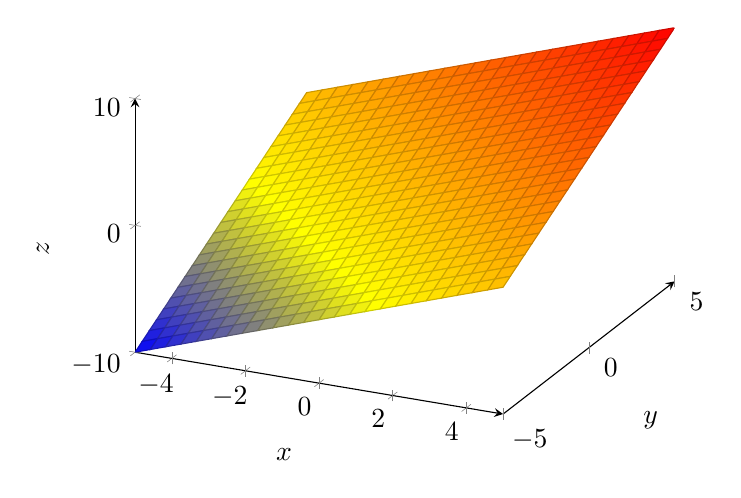
\begin{tikzpicture}
\begin{axis}[xlabel=$x$,ylabel=$y$,zlabel=$z$,axis lines=left,
  xlabel style={name=xl},ylabel style={name=yl},zlabel style={name=zl}]
\addplot3[surf] {x+y};
\coordinate (origin) at (axis description cs:0,0);
\coordinate (extent) at (axis description cs:1,1);
\end{axis}
\typeout{CASE default-left}\report
\end{tikzpicture}
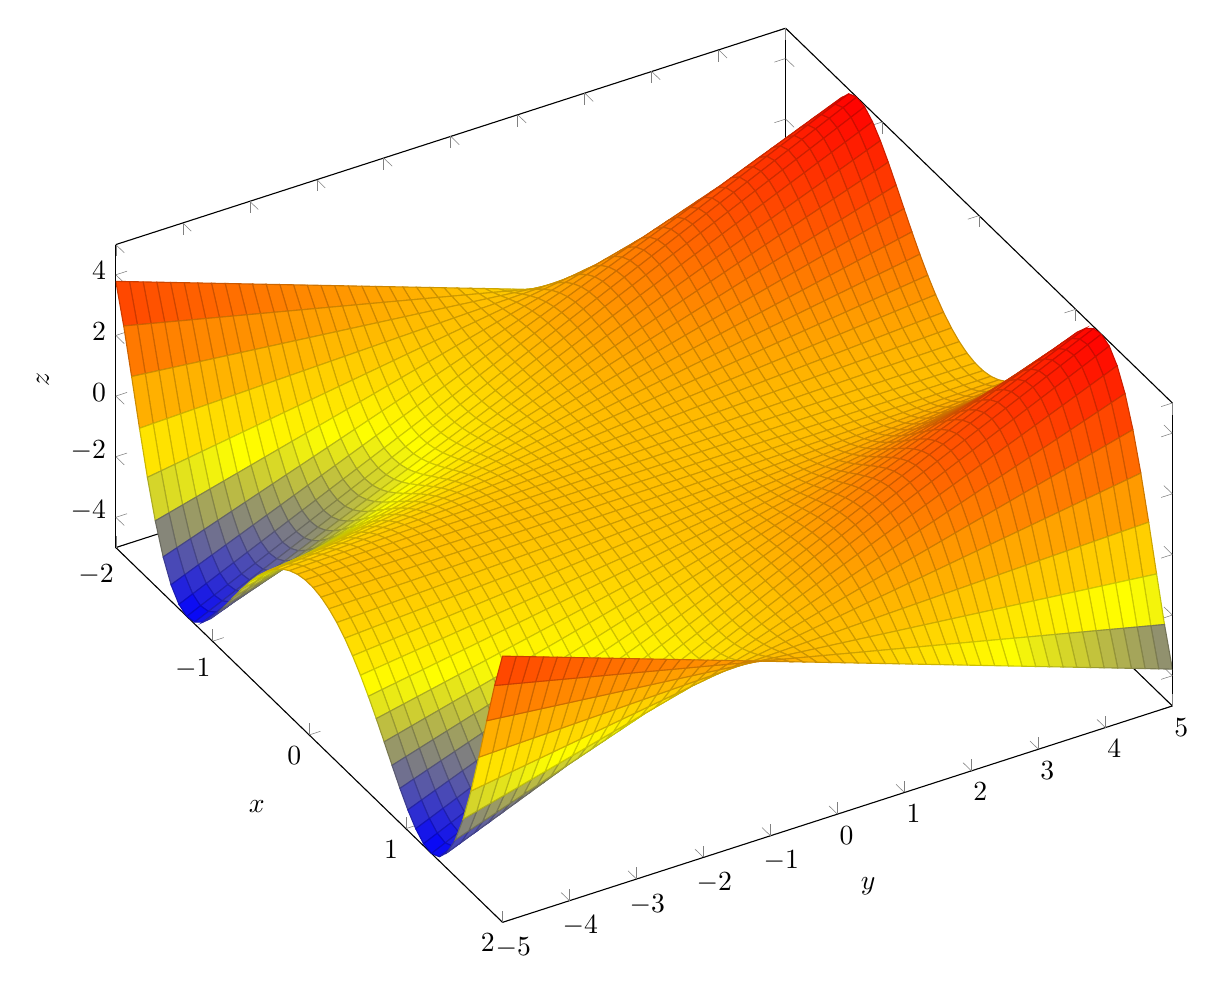
\begin{tikzpicture}
\begin{axis}[width=15cm,view={60}{55},enlargelimits=false,domain=-2:2,y domain=-5:5,samples=50,
  xlabel=$x$,ylabel=$y$,zlabel=$z$,xlabel style={name=xl},ylabel style={name=yl},zlabel style={name=zl}]
\addplot3[surf] {sin((x*x)r)*y};
\coordinate (origin) at (axis description cs:0,0);
\coordinate (extent) at (axis description cs:1,1);
\end{axis}
\typeout{CASE sinusoidal-ridge}\report
\end{tikzpicture}
\end{document}
